\documentclass[11pt]{article}
\usepackage{times}
\usepackage{graphicx}
\usepackage{hyperref}
\usepackage[margin=1in]{geometry}
\usepackage{amsmath}

\hypersetup{
	colorlinks=true,
	linkcolor=blue,
	filecolor=magenta,
	urlcolor=cyan,
}

\begin{document}

%===================================================
% Title and Author Info
%===================================================
\begin{center}
{\Large\textsc{Newtonian Tidal Effects and Neutron Star Inspiral}} \\
\vspace{10pt}
{\large Alex Urban} \\
{\small LIGO Laboratory, California Institute of Technology \\
Pasadena, CA 91125, USA \\
\href{mailto:aurban@ligo.caltech.edu}{aurban@ligo.caltech.edu}}
\end{center}

\section{Problem}
Suppose that a neutron star binary (each with mass $M = 1.4\,\, M_{\odot}$) is in a stable, Keplerian orbit (\textit{i.e.} with no loss of energy). Figure \ref{fig:binary_diagram} illustrates this system.

\begin{enumerate}
\item Compute the separation (in km) between the stars in terms of the gravitational wave frequency.

\item Compute the gravitational force between star 1 and a chunk of mass on the near side of star 2, and again for a chunk on the far side of star 2. Compare this, quantitatively, to the force binding those two chunks to their own star 2. Make a plot of these quantities, vs the gravitational wave frequency.”
\end{enumerate}

\subsection*{Solution}

\begin{enumerate}

\item From Kepler's third law, we can relate the orbital period ($P_{\rm orbital}$) and the orbital separation ($a$):
\[
\frac{P^2_{\rm orbital}}{a^3} = \frac{4\pi^2}{2GM}.
\]
We also know that gravitational waves from this system radiate at twice the orbital frequency, $f_{\rm GW} = 2f_{\rm orbital} = 2/P_{\rm orbital}$, so we can solve for $a$ with a bit of algebra:
\begin{equation}
a = \left[ \frac{2GM}{(\pi f_{\rm GW})^2} \right]^{1/3}.
\end{equation}
That effectively solves the first part.

\item From Newton's law of universal gravitation, we know that the force felt by star 2 due to star 1 on the near side is
\begin{equation}
F_{\rm near} = -\frac{GM^2}{(a - R)^2}
\end{equation}
where $R$ is the neutron star radius. Similarly, the force felt on the far side is
\begin{equation}
F_{\rm far} = -\frac{GM^2}{(a + R)^2}.
\end{equation}
The difference between these is the tidal force:
\begin{equation}
F_{\rm tidal} = F_{\rm near} - F_{\rm far} = GM^2 \left( \frac{1}{(a - R)^2} - \frac{1}{(a + R)^2} \right)
\end{equation}
When the tidal force overcomes the gravitational self-force of the neutron star,
\begin{equation}
F_{\rm self} = \frac{GM^2}{R^2},
\end{equation}
we know the star will start to be destroyed. Figure \ref{fig:NS_tides} illustrates this process for different neutron star radii, in terms of the gravitational wave frequency.

\end{enumerate}

\begin{figure}
\centering
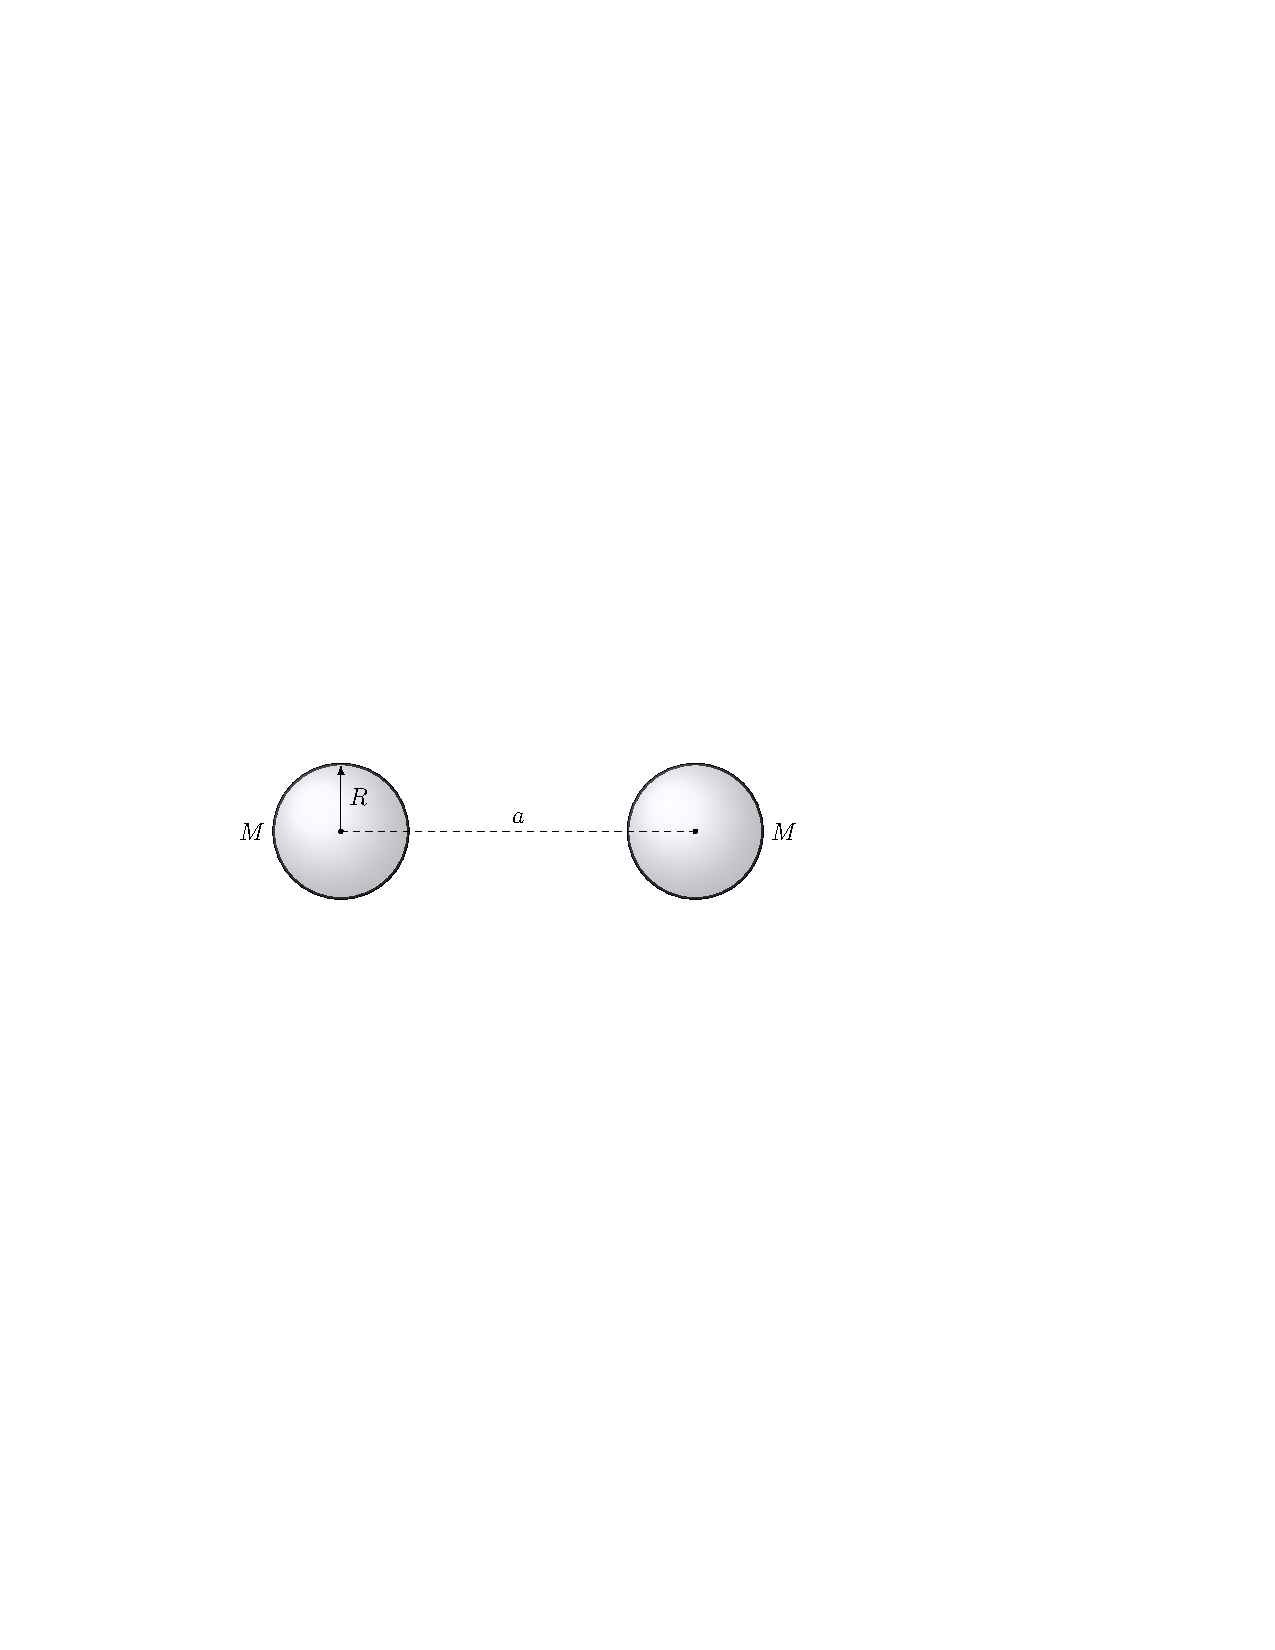
\includegraphics{binary_diagram.pdf}
\caption{\label{fig:binary_diagram}Diagram of the neutron star binary, showing its orbital separation ($a$) and the radius ($R$) and masses ($M$) of the individual neutron stars.}
\end{figure}

\begin{figure}
\centering
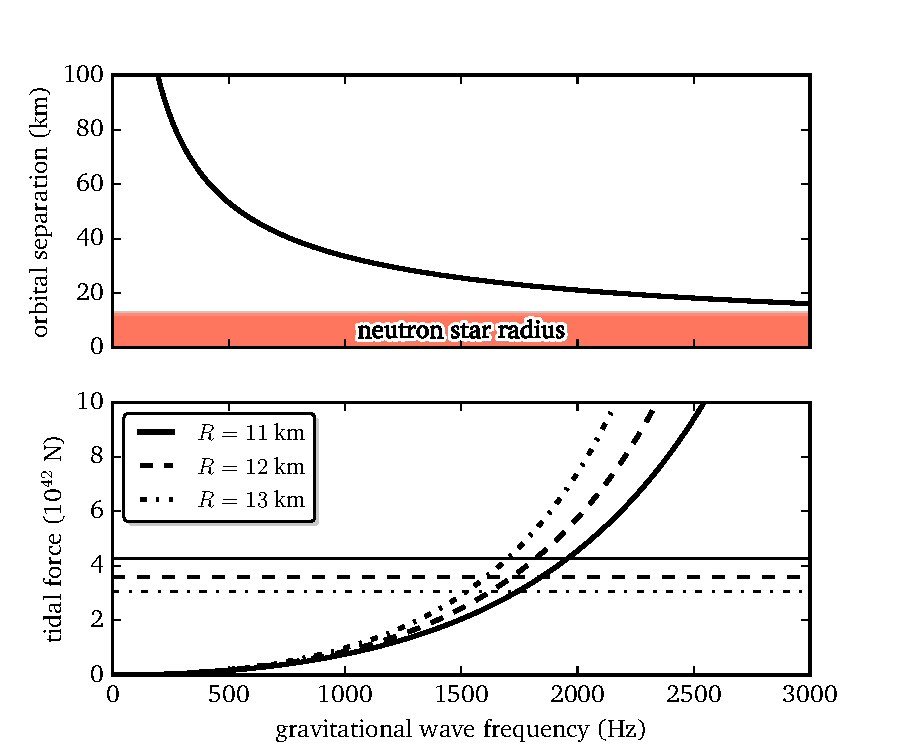
\includegraphics[scale=0.5]{newtonian_tidal_forces.pdf}
\caption{\label{fig:NS_tides}Top: the orbital separation (in km) between two neutron stars as a function of gravitational wave frequency. Bottom: The tidal forces (in Newtons) on one neutron star due to the other, compared at different neutron star radii. The horizontal lines show the neutron star's total binding force -- when the tidal force exceeds this, the neutron star will be ripped to smitherines in an absolutely epic lightshow.}
\end{figure}

\end{document}
